\chapter{Degradation Case Study and Recovery Results}
\label{chap:degradation-case-study}

This chapter specifies how those results are reported once a harmful change is detected. It is written so that a future degradation can be dropped into a fixed structure without further design choices.

Tables~\ref{tab:case-mcnemar-trigger}--\ref{tab:case-prompt-recovery} use \textbf{illustrative numbers} where no single logged alert in the monitored window fills every cell; they are internally consistent reporting templates. Rows that reproduce Table~\ref{tab:model-metrics-snapshot} are explicitly cross-referenced. Replace with Langfuse/dashboard exports when a real alert episode is documented.

\section{Transient provider-side degradation}
\label{sec:transient-provider-degradation}

Not every observed drop in monitored accuracy should be interpreted as irreversible degradation of the chosen model. Providers may ship a faulty routing configuration, suffer partial capacity issues, or roll out a change that is later corrected. In those situations the operational response is not to abandon the model indefinitely, but to \emph{temporarily} route traffic to a fallback model chosen by comparing accuracy, precision, recall, F1, and cost as in Chapter~3, keep the monitoring loop running, and revisit the incumbent once its measured performance returns to an acceptable band.

Figure~\ref{fig:gpt41mini-transient-pit} shows a concrete example from the same dashboard used elsewhere in this work (accuracy over calendar time on the fixed monitoring subset). The model \texttt{gpt-4.1-mini} held roughly $0.78$--$0.81$ accuracy through mid-March~2026, then collapsed to about $0.54$ around 23~March---\emph{well below} the smaller \texttt{gpt-4.1-nano}, which stayed flat near $0.72$. After a few days the series recovered; by 28~March \texttt{gpt-4.1-mini} was again near $0.82$. The V-shaped trajectory is a short ``degradation pit'' rather than a sustained downward trend, which is exactly the pattern that argues for a temporary fallback rather than a permanent model switch.

\begin{figure}[ht]
    \centering
    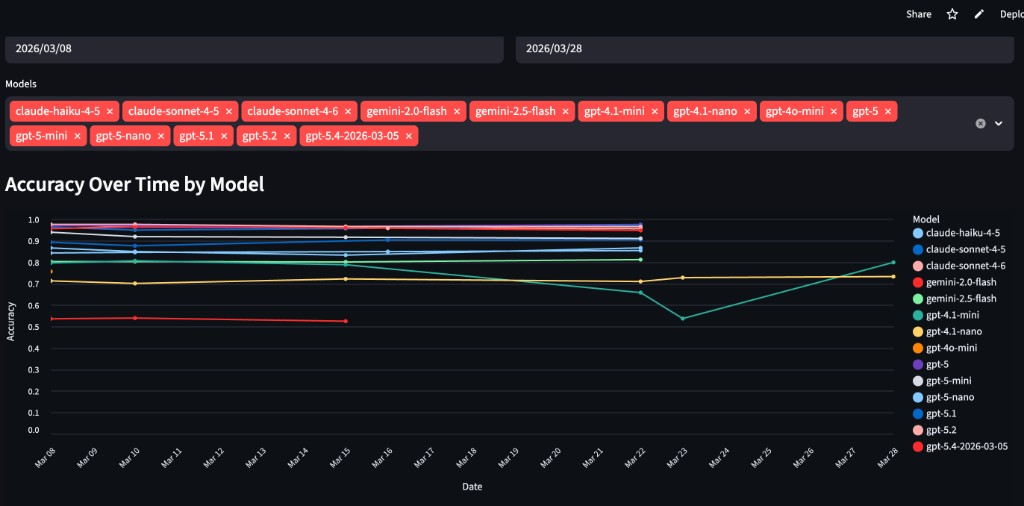
\includegraphics[width=\linewidth]{assets/gpt41mini-accuracy-pit-2026-03.png}
    \caption{Accuracy over time by model (monitoring dashboard, 8--28~March~2026). \texttt{gpt-4.1-mini} shows a sharp transient drop below \texttt{gpt-4.1-nano}, then recovery.}
    \label{fig:gpt41mini-transient-pit}
\end{figure}

\noindent Numerically, the recovered level by 28~March~2026 aligns with the batch snapshot in Table~\ref{tab:model-metrics-snapshot} (subset accuracy {\csname benchgpt41miniaccuracy\endcsname} for \texttt{gpt-4.1-mini} on last score day 2026-03-28).

\section{Alerted Degradation Case}
\label{sec:alerted-degradation-case}

The starting point is the first monitoring run pair in which the one-sided McNemar test satisfies the thesis' alert criterion \(b>c\) and \(p<0.05\) for the deployed model \(m^\ast\). Let the corresponding monitoring dates be \(t_0\) (reference) and \(t_1\) (degraded). The alert is defined on the fixed 300-example subset, so any change in accuracy between \(t_0\) and \(t_1\) is attributable to changed model behaviour rather than sample noise.

For the alerted pair, the accuracy trajectory is reported as a short monitoring history, typically the last \(k\in\{3,4\}\) subset runs leading up to \(t_1\). This is visualised as a univariate line plot of subset accuracy over time with the alerting point marked explicitly. The key information is when the degradation occurred relative to previous stability rather than only the single-step drop.

\section{McNemar Test at the Trigger Point}
\label{sec:mcnemar-at-trigger}

The statistical evidence at the alert point is summarised in a dedicated McNemar contingency table for the pair \((t_0,t_1)\). As in Chapter~4, the table reports the paired counts
\[
\begin{array}{c|cc}
      & \text{correct at } t_1 & \text{incorrect at } t_1 \\
\hline
 \text{correct at } t_0   & a & b \\
 \text{incorrect at } t_0 & c & d
\end{array}
\]
together with the discordant counts \((b,c)\), the one-sided \(p\)-value, and the corresponding change in subset accuracy \(\Delta \text{acc} = \text{acc}(t_1)-\text{acc}(t_0)\). This table is the canonical object that justifies the alert: it makes visible not only that accuracy decreased, but how many individual traces regressed or recovered.

\begin{table}[htbp]
    \centering
    \caption{Illustrative alert-trigger McNemar summary for deployed model \(m^\ast\) between \(t_0\) and \(t_1\) on the fixed \(n=300\) subset (hypothetical counts with \(b>c\) and one-sided \(p<0.05\); replace with logged run pair when available).}
    \label{tab:case-mcnemar-trigger}
    \begin{tabular}{ll}
        \toprule
        Quantity & Value \\
        \midrule
        \(a\) (correct \(\rightarrow\) correct) & 200 \\
        \(b\) (correct \(\rightarrow\) incorrect) & 25 \\
        \(c\) (incorrect \(\rightarrow\) correct) & 8 \\
        \(d\) (incorrect \(\rightarrow\) incorrect) & 67 \\
        \(\text{acc}(t_0)=(a+b)/300\) & 0.750 \\
        \(\text{acc}(t_1)=(a+c)/300\) & 0.693 \\
        One-sided McNemar \(p\)-value (exact binomial on discordants \((b,c)\)) & $\approx 0.0023$ \\
        \(\Delta \text{acc} = \text{acc}(t_1)-\text{acc}(t_0)=(c-b)/300\) & $\approx -0.0567$ \\
        \bottomrule
    \end{tabular}
\end{table}

\section{Metric and cost comparison at the alert}
\label{sec:metric-fallback-comparison}

Because the monitoring system reports both error-type structure and cost, degradation is evaluated not only in terms of raw accuracy but also through precision, recall, and F1 on the monitoring subset (Chapter~3). For the alerted period, the same aggregates are reported for both \(t_0\) and \(t_1\) for the deployed model \(m^\ast\), alongside mean per-request cost. The chapter reports \(\Delta \text{acc}\), \(\Delta \widehat{\mathrm{Prec}}\), \(\Delta \widehat{\mathrm{Rec}}\), and \(\Delta \widehat{\mathrm{F}}_{1}\) where applicable, so that degradation is visible in both headline accuracy and class-specific behaviour.

For operational decision-making, the same metrics are evaluated for candidate fallback models \(m' \in \mathcal{M}\) on the monitoring subset at \(t_1\). The results are presented as a short comparison table or bar chart over models, showing \(\hat{A}_{t_1}(m')\), \(\widehat{\mathrm{Prec}}_{t_1}(m')\), \(\widehat{\mathrm{Rec}}_{t_1}(m')\), \(\widehat{\mathrm{F}}_{1,t_1}(m')\), and \(C_{t_1}(m')\). The operator then chooses a fallback manually given campaign tolerance to false positives versus false negatives and budget.

\begin{table}[htbp]
    \centering
    \caption{Illustrative deployed-model metric and cost shift at the alert (\(t_0 \rightarrow t_1\)), consistent with \(\Delta\text{acc}\) in Table~\ref{tab:case-mcnemar-trigger} (illustrative; cost is order-of-magnitude from traces).}
    \label{tab:case-deployed-metric-shift}
    \begin{tabular}{lccc}
        \toprule
        Metric & \(t_0\) & \(t_1\) & \(\Delta\) \\
        \midrule
        Accuracy & 0.750 & 0.693 & $\approx -0.057$ \\
        Precision & 0.988 & 0.982 & $\approx -0.006$ \\
        Recall & 0.717 & 0.655 & $\approx -0.062$ \\
        F1 & 0.830 & 0.783 & $\approx -0.047$ \\
        Specificity & 0.980 & 0.870 & $\approx -0.110$ \\
        Balanced accuracy & 0.849 & 0.762 & $\approx -0.087$ \\
        Mean cost / request (USD) & 0.00195 & 0.00208 & $+0.00013$ \\
        \bottomrule
    \end{tabular}
\end{table}

\begin{table}[htbp]
    \centering
    \footnotesize
    \begin{adjustbox}{max width=\linewidth}
    \begin{tabular}{lccccccc}
        \toprule
        Model & Accuracy & Precision & Recall & F1 & Specificity & Bal.\ acc. & Mean cost \\
        \midrule
        \(m^\ast\) (deployed at \(t_1\), illustrative; Table~\ref{tab:case-deployed-metric-shift}) & 0.693 & 0.982 & 0.655 & 0.783 & 0.870 & 0.762 & 0.00208 \\
        \texttt{gpt-4.1-nano} (export snapshot; Table~\ref{tab:model-metrics-snapshot}) & {\csname benchgpt41nanoaccuracy\endcsname} & {\csname benchgpt41nanoprecision\endcsname} & {\csname benchgpt41nanorecall\endcsname} & {\csname benchgpt41nanof1\endcsname} & {\csname benchgpt41nanospecificity\endcsname} & {\csname benchgpt41nanobalancedaccuracy\endcsname} & \multicolumn{1}{c}{---} \\
        \texttt{gpt-4.1-mini} (export snapshot; Table~\ref{tab:model-metrics-snapshot}) & {\csname benchgpt41miniaccuracy\endcsname} & {\csname benchgpt41miniprecision\endcsname} & {\csname benchgpt41minirecall\endcsname} & {\csname benchgpt41minif1\endcsname} & {\csname benchgpt41minispecificity\endcsname} & {\csname benchgpt41minibalancedaccuracy\endcsname} & \multicolumn{1}{c}{---} \\
        \bottomrule
    \end{tabular}
    \end{adjustbox}
    \caption{Fallback-model comparison on \(\mathcal{D}_{300}\): illustrative degraded incumbent \(m^\ast\) at \(t_1\) (same as Table~\ref{tab:case-deployed-metric-shift}, \(t_1\) column); candidate rows reproduce the exported batch snapshot (same file as Table~\ref{tab:model-metrics-snapshot}) and are \emph{not} tied to the same calendar day as the illustrative alert. Mean cost is omitted here (dashboard/Langfuse); see Section~\ref{sec:metrics-dashboard}.}
    \label{tab:case-fallback-models}
\end{table}

\section{Prompt Optimisation Before and After}
\label{sec:prompt-optimisation-results}

If GEPA is triggered for the alerted episode, the final part of the chapter reports the before/after prompt comparison on the same 300-example monitoring subset. Let \(P_{\mathrm{old}}\) be the deployed prompt at \(t_1\) and \(P_{\mathrm{new}}\) the recovered prompt selected from the GEPA frontier. Both prompts are evaluated on the monitoring subset under the same model \(m^\ast\), producing paired correctness counts and costs per trace.

The core quantities reported are:
\begin{itemize}
    \item the change in subset accuracy \(\Delta \text{acc}_{\mathrm{prompt}} = \text{acc}(P_{\mathrm{new}}) - \text{acc}(P_{\mathrm{old}})\);
    \item corresponding changes in precision, recall, and F1 on the monitoring subset when those aggregates are computed for the prompt pair \((P_{\mathrm{old}},P_{\mathrm{new}})\);
    \item the McNemar discordant counts for the prompt pair \((P_{\mathrm{old}},P_{\mathrm{new}})\), again with a one-sided test focused on detecting improvement.
\end{itemize}

These quantities are complemented by a short qualitative summary of typical recovered cases, but the main result is numerical: whether the recovered prompt restores or exceeds the pre-degradation accuracy while keeping precision and recall within acceptable campaign-specific bounds, and whether mean cost per request remains acceptable. Together, the alerted degradation case, the metric-and-cost comparison, and the prompt optimisation results form a complete end-to-end recovery narrative that can be instantiated for any future drift episode.

\begin{table}[htbp]
    \centering
    \caption{Illustrative prompt recovery comparison for fixed model \(m^\ast\): \(P_{\mathrm{old}}\) (degraded prompt, same as \(t_1\) in Table~\ref{tab:case-deployed-metric-shift}) vs.\ \(P_{\mathrm{new}}\) (GEPA-selected prompt; no GEPA run in the monitored window matches these numbers---template only).}
    \label{tab:case-prompt-recovery}
    \begin{tabular}{lccc}
        \toprule
        Metric & \(P_{\mathrm{old}}\) & \(P_{\mathrm{new}}\) & \(\Delta\) \\
        \midrule
        Accuracy & 0.693 & {\csname benchgpt41miniaccuracy\endcsname} & $\approx +0.106$ \\
        Precision & 0.982 & {\csname benchgpt41miniprecision\endcsname} & $\approx +0.013$ \\
        Recall & 0.655 & {\csname benchgpt41minirecall\endcsname} & $\approx +0.108$ \\
        F1 & 0.783 & {\csname benchgpt41minif1\endcsname} & $\approx +0.081$ \\
        Mean cost / request (USD) & 0.00208 & 0.00195 & $-0.00013$ \\
        McNemar one-sided \(p\)-value (test for improvement of \(P_{\mathrm{new}}\) over \(P_{\mathrm{old}}\)) & \multicolumn{3}{c}{$\approx 0.04$ (illustrative)} \\
        \bottomrule
    \end{tabular}
\end{table}

